% Figura Anexo II: los dos mecanismos de transmisión monetaria: (a) keynesiano; (b) monetarista
\documentclass[tikz,border=3pt]{standalone}
\usepackage[T1]{fontenc}
\usepackage[utf8]{inputenc}
\usetikzlibrary{arrows.meta,calc,positioning}
\begin{document}
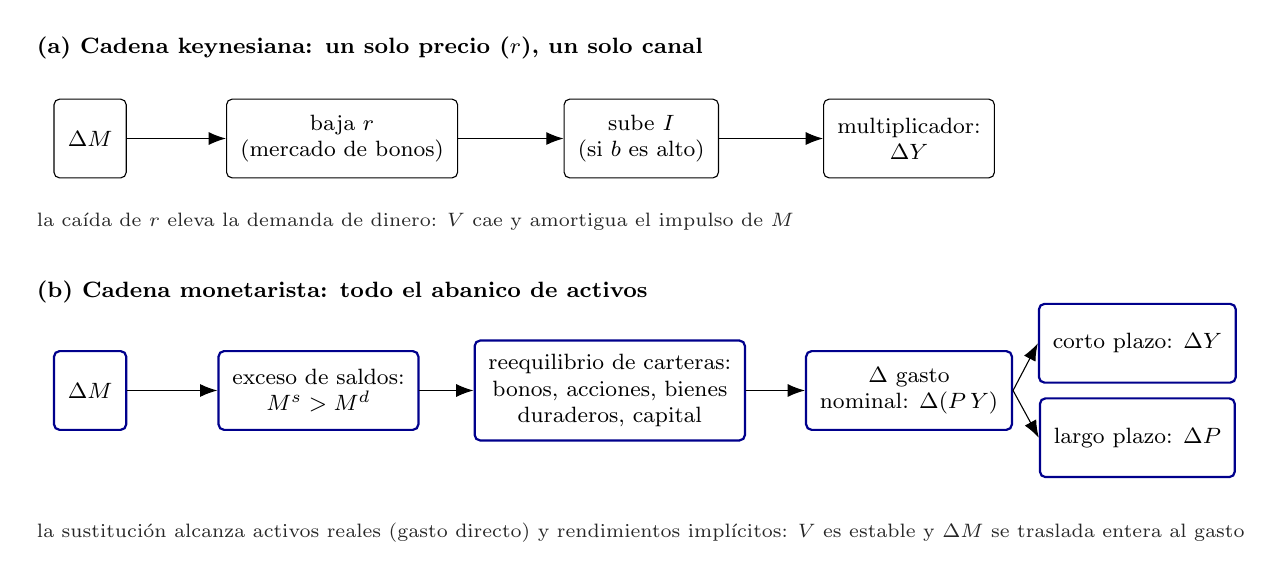
\begin{tikzpicture}[>={Latex[length=2.2mm]}, line cap=round, font=\footnotesize,
  caja/.style={draw, rounded corners=2pt, align=center, inner sep=5pt, minimum height=10mm},
  cajam/.style={draw=blue!55!black, thick, rounded corners=2pt, align=center, inner sep=5pt, minimum height=10mm}]
  % ---------- (a) cadena keynesiana ----------
  \node[font=\footnotesize\bfseries, anchor=west] at (-0.8,1.15) {(a) Cadena keynesiana: un solo precio ($r$), un solo canal};
  \node[caja] (k1) at (0,0) {$\Delta M$};
  \node[caja] (k2) at (3.2,0) {baja $r$\\(mercado de bonos)};
  \node[caja] (k3) at (7.0,0) {sube $I$\\(si $b$ es alto)};
  \node[caja] (k4) at (10.4,0) {multiplicador:\\$\Delta Y$};
  \draw[->] (k1) -- (k2);
  \draw[->] (k2) -- (k3);
  \draw[->] (k3) -- (k4);
  \node[anchor=west, gray!30!black] at (-0.8,-1.05) {\scriptsize la caída de $r$ eleva la demanda de dinero: $V$ cae y amortigua el impulso de $M$};
  % ---------- (b) cadena monetarista ----------
  \node[font=\footnotesize\bfseries, anchor=west] at (-0.8,-1.95) {(b) Cadena monetarista: todo el abanico de activos};
  \node[cajam] (m1) at (0,-3.2) {$\Delta M$};
  \node[cajam] (m2) at (2.9,-3.2) {exceso de saldos:\\$M^{s}>M^{d}$};
  \node[cajam] (m3) at (6.6,-3.2) {reequilibrio de carteras:\\bonos, acciones, bienes\\duraderos, capital};
  \node[cajam] (m4) at (10.4,-3.2) {$\Delta$ gasto\\nominal: $\Delta(P\,Y)$};
  \node[cajam] (m5a) at (13.3,-2.6) {corto plazo: $\Delta Y$};
  \node[cajam] (m5b) at (13.3,-3.8) {largo plazo: $\Delta P$};
  \draw[->] (m1) -- (m2);
  \draw[->] (m2) -- (m3);
  \draw[->] (m3) -- (m4);
  \draw[->] (m4.east) -- (m5a.west);
  \draw[->] (m4.east) -- (m5b.west);
  \node[anchor=west, gray!30!black] at (-0.8,-5.0) {\scriptsize la sustitución alcanza activos reales (gasto directo) y rendimientos implícitos: $V$ es estable y $\Delta M$ se traslada entera al gasto};
\end{tikzpicture}
\end{document}
